\section{Theorie}


\subsection{Stubfilter}

LC-Filter können in einem weiten Frequenzbereich eingesetzt werden. Jedoch wird bei konzentrierten Elementen zu höheren Frequenzen hin der Einfluss der parasitären Eigenschaften immer deutlicher, so dass hohe Anaforderungen an die Bauteilgüte gestellt werden müssen. Im GHZ-Bereich wird es daher zunehmend attraktiv, statt konzentrierten Kapazitäte und Induktivitäten verteilte Strukturen in Form von Leitungen zu verwenden.
%Quelle direktes Zitat: 
%https://books.google.ch/books?id=MTVQAgAAQBAJ&pg=PA203&lpg=PA203&dq=leitungsfilter+hochfrequenztechnik&source=bl&ots=Ljf0GRJkZt&sig=n-0G9H5VZ9iuPc2qepAATnjA47M&hl=de&sa=X&ved=0ahUKEwj38u-T79DUAhUSL1AKHUsyDNMQ6AEINTAB#v=onepage&q=leitungsfilter%20hochfrequenztechnik&f=false%

Es gibt verschiedene Arten um Leitungsfilter zu realisieren. Eine Möglichkeit der Realisierung ist das Stubfilter. Dieses Filter verwendet gleichlange kurzgeschlossenen Leitungen (TLSC) und leerlaufende Leitungen(TLOC), die nur an einem Ende verbunden werden. Das andere Ende wird kurzgeschlossen oder offen gelassen. Man spricht in diesem Fall von sogennanten Stubs(Stichleitungen), die sich bei hohen Frequenzen wie reaktive Elemente (L,C) verhalten und somit die  Realisierung eines Mikrowellenfilter ermöglichen. Der grosse Vorteil ist das eine geschlossene Theorie existiert, welche die Synthese von Stubfiltern ermöglicht.


\subsection{Ablauf Stubfilterdimensionierung}
In diesem Kapitel wird erläutert, wie bei der Dimensionierung eines Stubfilters  vorgegangen wird. Der typische Ablauf zur Dimensionierung eines Stubfiltern ist in Abb. \ref{fig:Ablauf_Filterdimensionierung dargestellt. Dieser Ablauf unterscheidet sich nicht gross vom Ablauf bei der Dimensionierung eines digitalen oder  Ablaufwird auch für die Realisierung von aktiven, passiven und digitalen Filters verwendet. Der einzige Unterschied ist, dass sich die Schritte in Filter-Realisierung(blau umrandet) unterscheiden.

Ausgangslage für jede Filterdimensionierung ist die Filterspezifikation, welche im Frequenz- oder Zeitbereich vorliegt. Diese Filterspezifikation wird anschliessen mathematisch mit einer Funktion in der s-Ebene (Prototypbereich) beschrieben. Mit einem Synthesetool kann aus der Funktion in der s-Ebene ein Prototypfilter mit konzentrierten Elementen(R,L,C) gefunden werden. Dabei gibt das Synthesetool die Topologie, sowie die Bauteilwerte aus. Liegt kein Synthesetool vor, so müssen Standardfilter (Butterworth, Chebyshev, Bessel und Cauer) verwendet werden, deren Topologie und Bauteilwerte normiert aus einer Tabelle zu entnehmen sind. Bei sehr speziellen Anforderungen an das Filter reichen die Standardfilter aber meist nicht aus um die Filterspezifikationen einzuhalten.

Nach der Synthese liegt nun ein Prototypfilter mit konzentrierten Elementen vor, gesucht ist aber ein Stubfilter, welches aus verteilten Elementen (Leitungen) besteht. Hier kommt die Frequenztransformation von Richards zum Zuge. Richards konnte zeigen, dass sich gleichlange, verlustlose Leitungen (TLSC,TLOC) gleich wie konzentrierte Elemente verhalten, wenn die folgende Transformation für die laplace variable verwendet wird.

s= dhsijdkh

Mit der Frequenztransformation von Richards kann dieses Filter vom Prototypbereich(s-Eben) in den Originalbereich (f-Ebene) transformiert werden. Dadurch werden die konzentrierten Elemente(L,C) in verteilte Elemente (Leitungen) umgewandelt. Dies 
TLSC = ideale, verlustlose Transmission Line im kurzschluss
TLOC = ideale, verlustlse Tranmissin Line im Leerlauf



\newpage

\begin{figure}[h!]
\centering
 	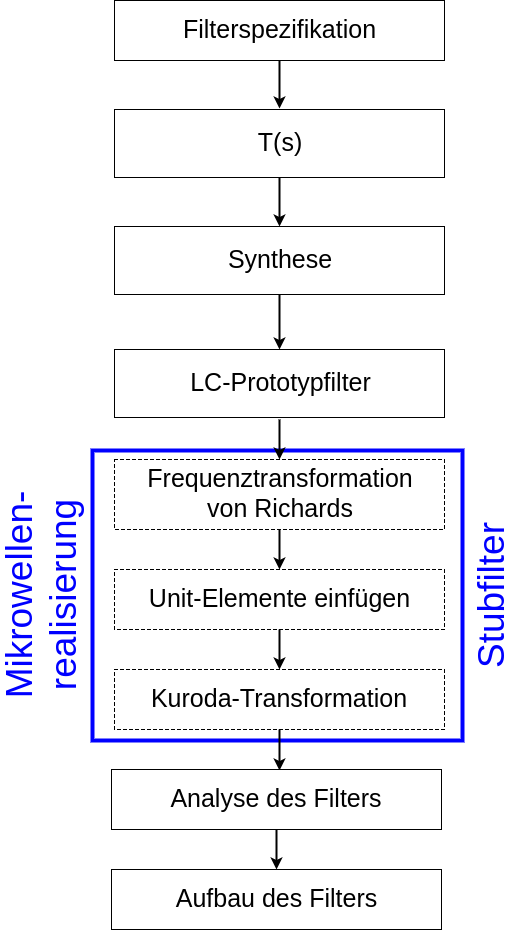
\includegraphics[width=0.5\textwidth]{Ablauf_Filterdimensionierung.png}
 	\caption{Ablauf der Stubfilter-Dimensionierung}
 	\label{fig:Ablauf_Filterdimensionierung}
\end{figure}
